\documentclass[25pt, a0paper, portrait]{tikzposter} %Options for format can be included here
\usepackage[]{amsmath}
\usepackage{helvet}
\renewcommand{\familydefault}{\sfdefault}

\definecolorstyle{Eucall}{%
  \definecolor{ECGreen}{HTML}{98CE7C}%
  \definecolor{ECYellow}{HTML}{F2E560}%
  \definecolor{ECYellowGreen}{HTML}{D6DA36}%
}%
{
  % Background Colors
  \colorlet{backgroundcolor}{white}
  \colorlet{framecolor}{black}
  % Title Colors
  \colorlet{titlefgcolor}{white}
  %\colorlet{titlebgcolor}{ECGreen!50!ECYellowGreen}
  \colorlet{titlebgcolor}{ECGreen}
  % Block Colors
  %\colorlet{blocktitlebgcolor}{ECGreen!50!ECYellowGreen}
  \colorlet{blocktitlebgcolor}{ECGreen}
  \colorlet{blocktitlefgcolor}{white}
  \colorlet{blockbodybgcolor}{white}
  \colorlet{blockbodyfgcolor}{black}
  % Innerblock Colors
  %\colorlet{innerblocktitlebgcolor}{ECYellowGreen!50!ECYellow}
  \colorlet{innerblocktitlebgcolor}{ECYellowGreen}
  \colorlet{innerblocktitlefgcolor}{black}
  \colorlet{innerblockbodybgcolor}{white}
  \colorlet{innerblockbodyfgcolor}{black}
  % Note colors
  \colorlet{notefgcolor}{black}
  %\colorlet{notebgcolor}{ECGreen!50!ECYellowGreen}
  \colorlet{notebgcolor}{ECGreen}
  \colorlet{noteframecolor}{black}
}

\definetitlestyle{Eucall}{%
    width=0.95\paperwidth, roundedcorners=30, linewidth=0.0cm, innersep=1cm,
    titletotopverticalspace=15mm, titletoblockverticalspace=20mm,
    titlegraphictotitledistance=0pt, titletextscale=1
}{%
    \begin{scope}[line width=\titlelinewidth, rounded corners=\titleroundedcorners]%
      \coordinate (bottomleft) at (\titleposleft+0.2\textwidth, \titleposbottom);%
      \coordinate (topright) at (\titleposright, \titlepostop);%
      \pgftext[right, x=\titleposleft+0.18\textwidth, y=0.5\titlepostop+0.5\titleposbottom]{
\includegraphics[width=0.18\textwidth]{eucall_logo}}%
      \draw[draw=none, left color=ECGreen, right color=ECYellowGreen](bottomleft) rectangle (topright);%
    \end{scope}%
}

\defineblockstyle{EucallLeft}{
    titlewidthscale=1, bodywidthscale=1, titleleft,
    titleoffsetx=0pt, titleoffsety=0pt, bodyoffsetx=25pt, %bodyoffsety=-10pt,
    bodyverticalshift=0pt, roundedcorners=30, linewidth=0.0cm,
    titleinnersep=1cm, bodyinnersep=1cm
}{%
    \begin{scope}[line width=\blocklinewidth, rounded corners=\blockroundedcorners]%
        \ifBlockHasTitle %
           \draw[draw=none, left color=ECGreen, right color=ECYellowGreen] (blocktitle.south west) rectangle (blocktitle.north east);
           \draw[draw=none, fill=blockbodybgcolor] (blockbody.south west) rectangle (blockbody.north east);
        \else
           \draw[draw=none, fill=blockbodybgcolor] (blockbody.south west) rectangle (blockbody.north east);
        \fi
    \end{scope}
}
\defineblockstyle{EucallCenter}{
    titlewidthscale=1, bodywidthscale=1, titleleft,
    titleoffsetx=0pt, titleoffsety=0pt, bodyoffsetx=25pt, bodyoffsety=-10pt,
    bodyverticalshift=0pt, roundedcorners=30, linewidth=0.0cm,
    titleinnersep=1cm, bodyinnersep=1cm
}{%
    \begin{scope}[line width=\blocklinewidth, rounded corners=\blockroundedcorners]%
        \ifBlockHasTitle %
           \draw[draw=none, fill=ECGreen] (blocktitle.south west) rectangle (blocktitle.north east);
           \draw[draw=none, fill=ECGreen] (blockbody.south west) rectangle (blocktitle.north east);
        \else
           \draw[draw=none, fill=blockbodybgcolor] (blockbody.south west) rectangle (blockbody.north east);
        \fi
    \end{scope}
}
\defineblockstyle{EucallRight}{
    titlewidthscale=1, bodywidthscale=1, titleleft,
    titleoffsetx=0pt, titleoffsety=0pt, bodyoffsetx=25pt, bodyoffsety=0pt,
    bodyverticalshift=0pt, roundedcorners=30, linewidth=0.0cm,
    titleinnersep=1cm, bodyinnersep=1cm
}{
    \begin{scope}[line width=\blocklinewidth, rounded corners=\blockroundedcorners]
        \ifBlockHasTitle %
           \draw[draw=none, left color=ECYellowGreen, right color=ECYellow] (blocktitle.south west) rectangle (blocktitle.north east);
           \draw[draw=none, color=blockbodybgcolor] (blockbody.south west) rectangle (blockbody.north east);
        \else
           \draw[draw=none, color=blockbodybgcolor] (blockbody.south west) rectangle (blockbody.north east);
        \fi
    \end{scope}
}



\definelayouttheme{Eucall}{%
  \usecolorstyle{Eucall}
  %\usecolorstyle{default}
  \usebackgroundstyle{Default}
  \usetitlestyle{Eucall}
  \useblockstyle{EucallLeft}
  \usenotestyle{Default}
}


% Switch off the tikz notice at the bottom
\tikzposterlatexaffectionproofoff

%%%%%%%%%%%%%%%%%%%%%%%%%%%%%%%%%%%%%%%%%%%%%%%%%%%%%%%%%%%%%%%%%%%%%%
%%% Begin of Document
%%%%%%%%%%%%%%%%%%%%%%%%%%%%%%%%%%%%%%%%%%%%%%%%%%%%%%%%%%%%%%%%%%%%%%


 % Title, Author, Institute
 \title{\hspace*{0.2\textwidth}\parbox{0.7\textwidth}{\centering\bf Simulation of Experiments for
 European Advanced Laser Light Sources}}
 \author{\hspace*{0.2\textwidth}{\parbox{0.7\textwidth}{\centering%
 C. Fortmann-Grote$^{1}$,
 A. Andreev$^\text{2}$,
 S. Aogaki$^\text{3}$,
 R. Briggs$^\text{4}$,
 M. Bussmann$^\text{5}$,
 M. Garten$^\text{5}$,
 M. Glass$^\text{4}$,
 A. Grund$^\text{5}$,
 A. H\"ubl$^\text{5}$,
 Y. Kemp$^\text{6}$,
 T. Kluge$^\text{5}$,\\
 A. P. Mancuso$^\text{1}$,
 S. Pascarelli$^\text{4}$,
 M. S\'anchez del R\'io$^\text{4}$,
 F. Schl\"unzen$^\text{6}$,\\
 S. Sternberger$^\text{6}$,
 R. Torchio$^\text{4}$,
 T. Vinci$^\text{7}$,
 J. Vorberger$^\text{5}$,
 R. Widera$^\text{5}$
 }}}
 \institute{\hspace*{0.2\textwidth}{\parbox{0.7\textwidth}{\centering\small%
 $^\text{1}$European XFEL, Hamburg, Germany,
 $^\text{2}$ELI-ALPS, Szeged, Hungary,
 $^\text{3}$ELI-NP, Bucharest, Romania,
 $^\text{4}$ESRF, Grenoble, France,
 $^\text{5}$HZDR, Dresden, Germany,\\
 $^\text{6}$DESY, Hamburg, Germany,
 $^\text{7}$LULI, Paris, France
 }}}

 %Choose Layout
\usetheme{Eucall}

\begin{document}

% Title block with title, author, logo, etc.
\maketitle
%%%
\begin{columns}
%%%%%%%%%%%%%%% FIRST column
\column{0.5}%
%%%
\block[bodyoffsetx=-20pt]{X-ray diffraction in underdense plasmas}{%
    \innerblock[titleleft, titleoffsetx=10pt,bodyoffsetx=10pt]
    {Identifying Plasma Instabilities by Small Angle X-Ray Scattering}
    {%
    \begin{minipage}[ ]{.95\colwidth}
      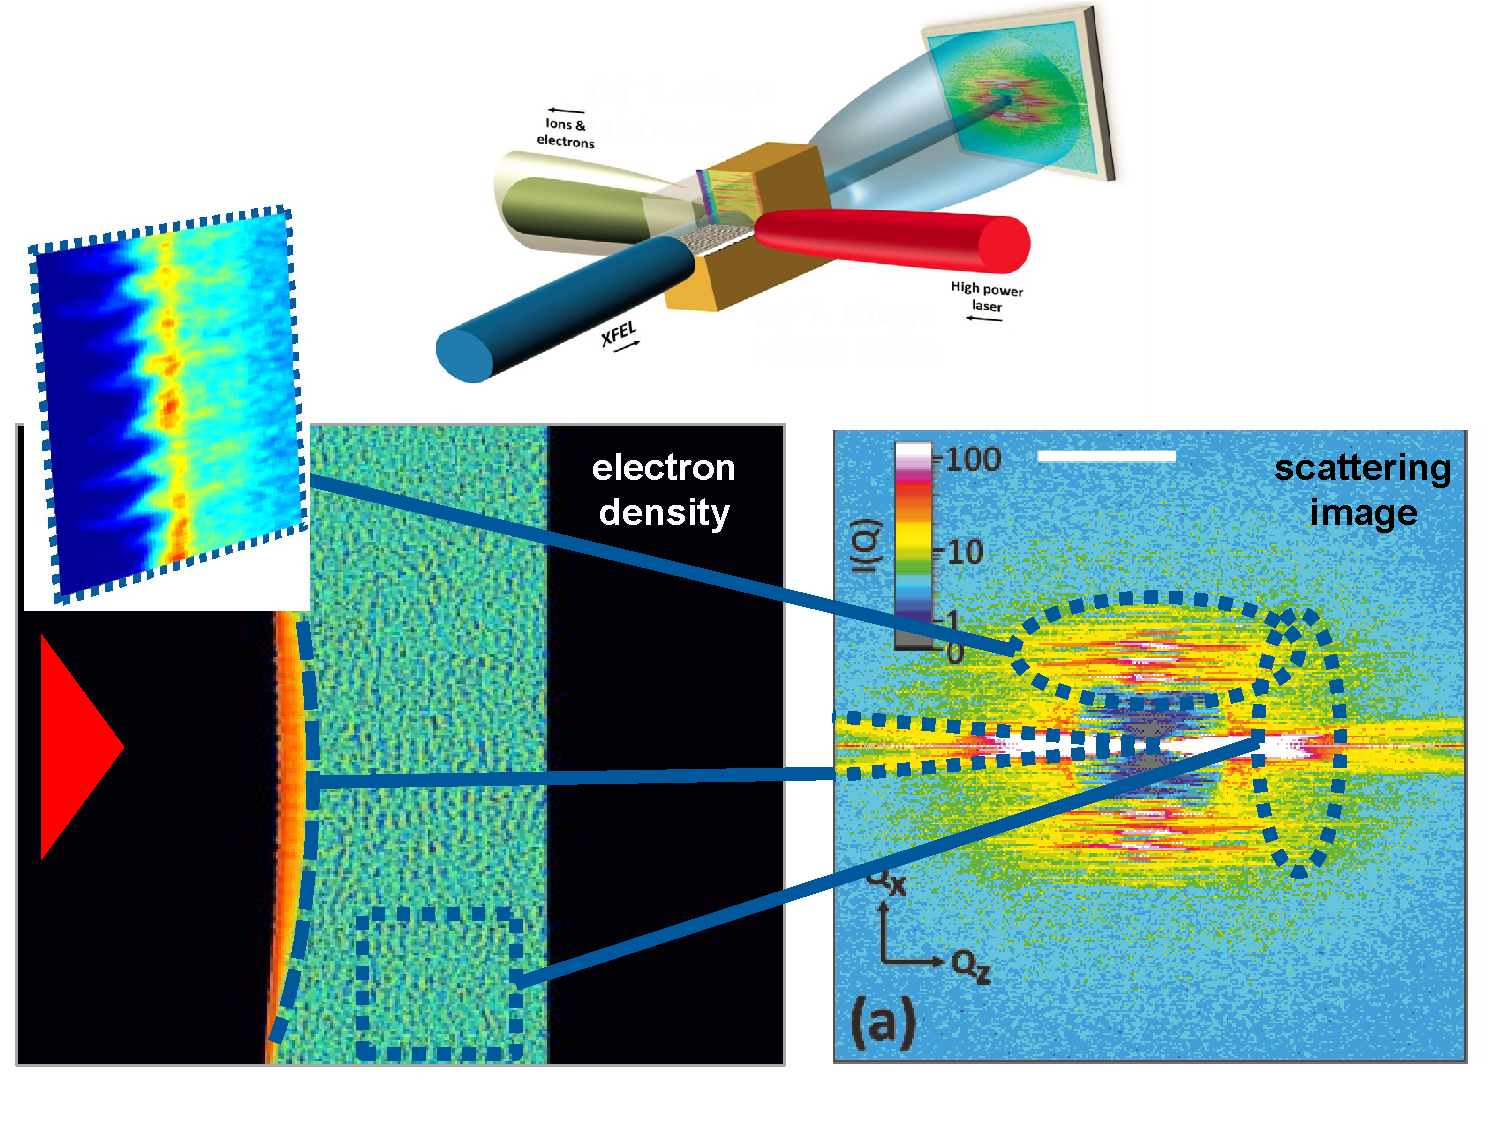
\includegraphics[width=.5\textwidth,angle=0,clip]{bussmann_saxs.pdf}%
      \hfill%
      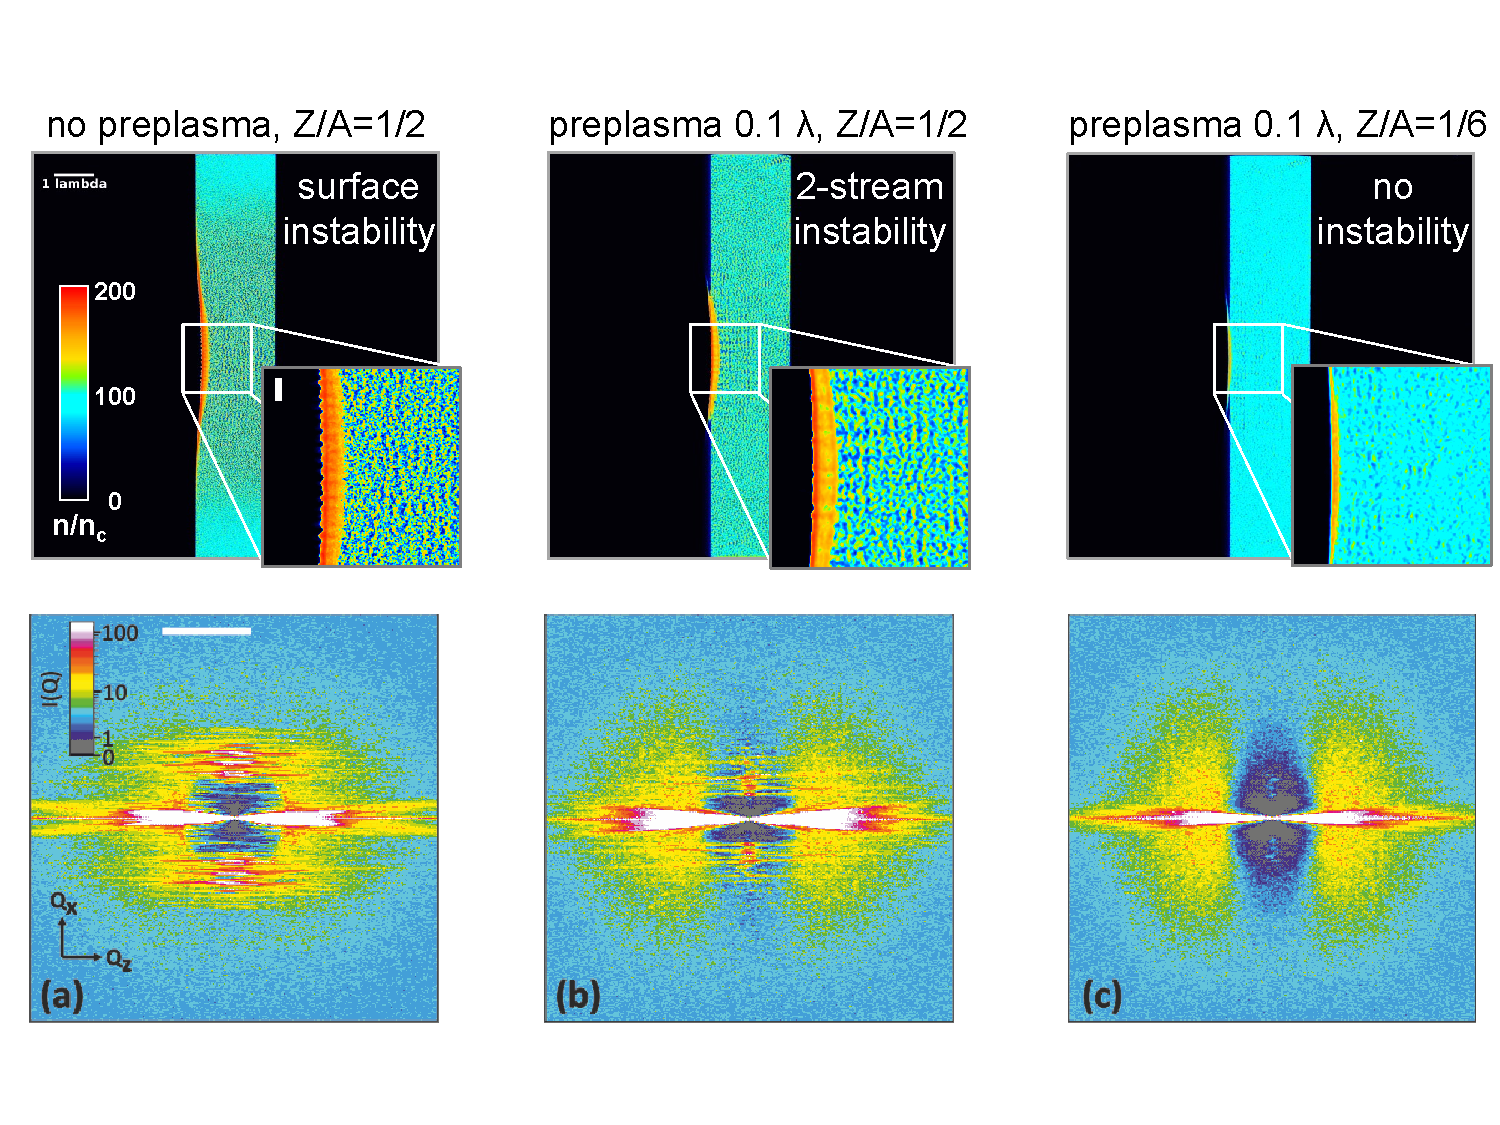
\includegraphics[width=.5\textwidth,angle=0,clip]{bussmann_saxs_instabilities.pdf}%
    \end{minipage}
    }%
    \vspace*{1ex}
    \innerblock[titleleft, titleoffsetx=10pt, bodyoffsetx=10pt]
    { Outlook: Combine PIC simulations [1] with population kinetics (scFLY [2])}
    {%
      \begin{minipage}[ ]{.9\colwidth}
        \mbox{}%
        \begin{minipage}[][][t]{.49\textwidth}
          \begin{center}
            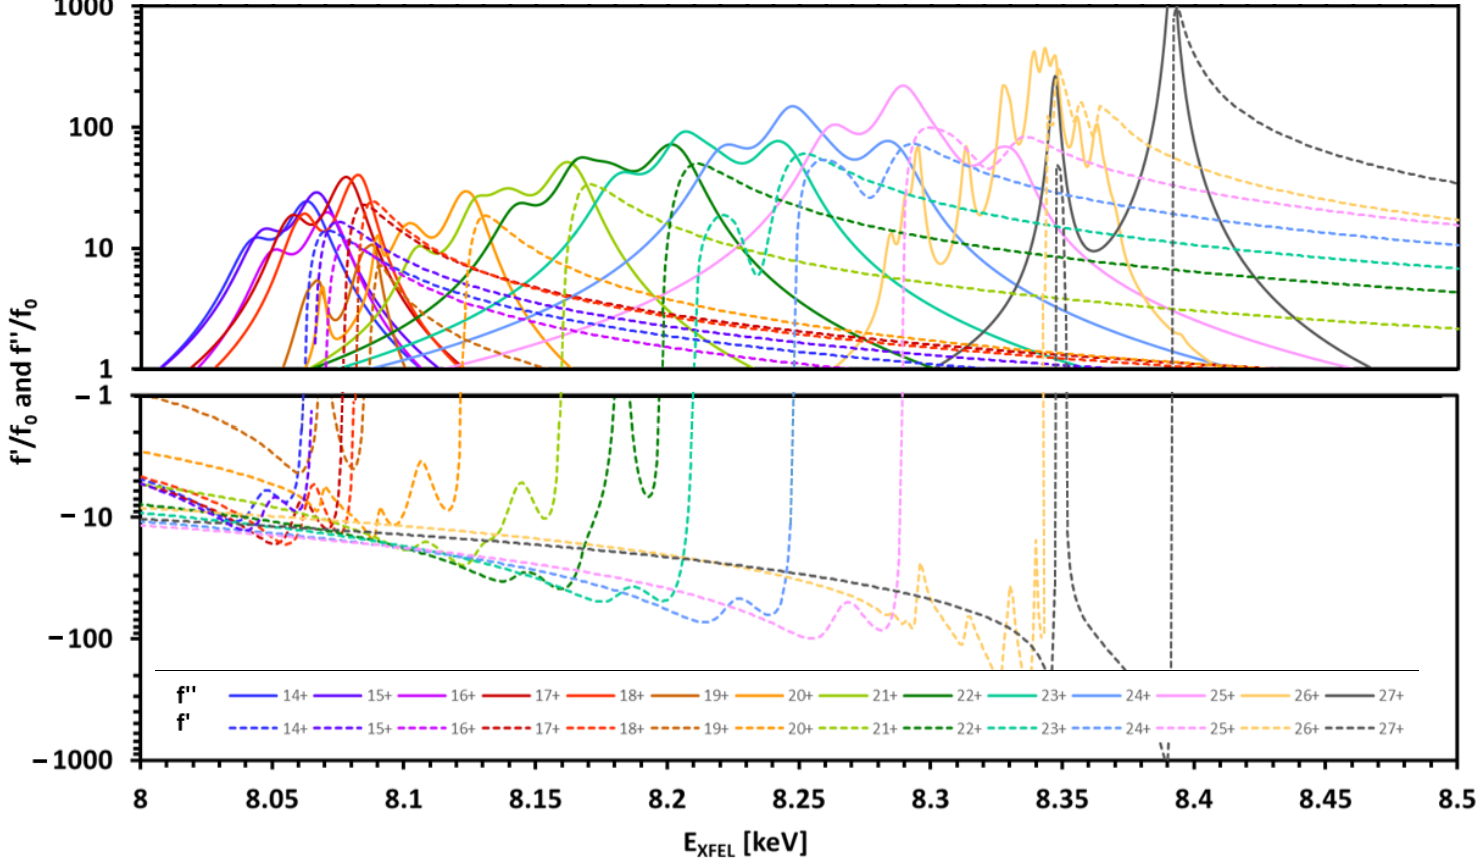
\includegraphics[width=.4\colwidth,angle=0,clip]{scfly.png}%
          \end{center}
        \end{minipage}
        \begin{minipage}[][][t]{.49\textwidth}
          \begin{itemize}
            \item Multiple photon scattering
            \item Atomic configurations
            \item Collisions
            \item Collisional and field ionization
            \item Radiation transport
            \item Recombination
          \end{itemize}
        \end{minipage}
      \end{minipage}
    }%
}%
\column{0.5}
\useblockstyle{EucallRight}
%%%
% ESRF WDM Diagnostics
\block[bodyoffsetx=-30pt]{X-ray diagnostics of Warm Dense Iron [3]}{%
  \innerblock[titleleft, titleoffsetx=10pt, bodyoffsetx=10pt]{Combining x-ray absorption spectroscopy with shock compression}{
  \begin{center}
    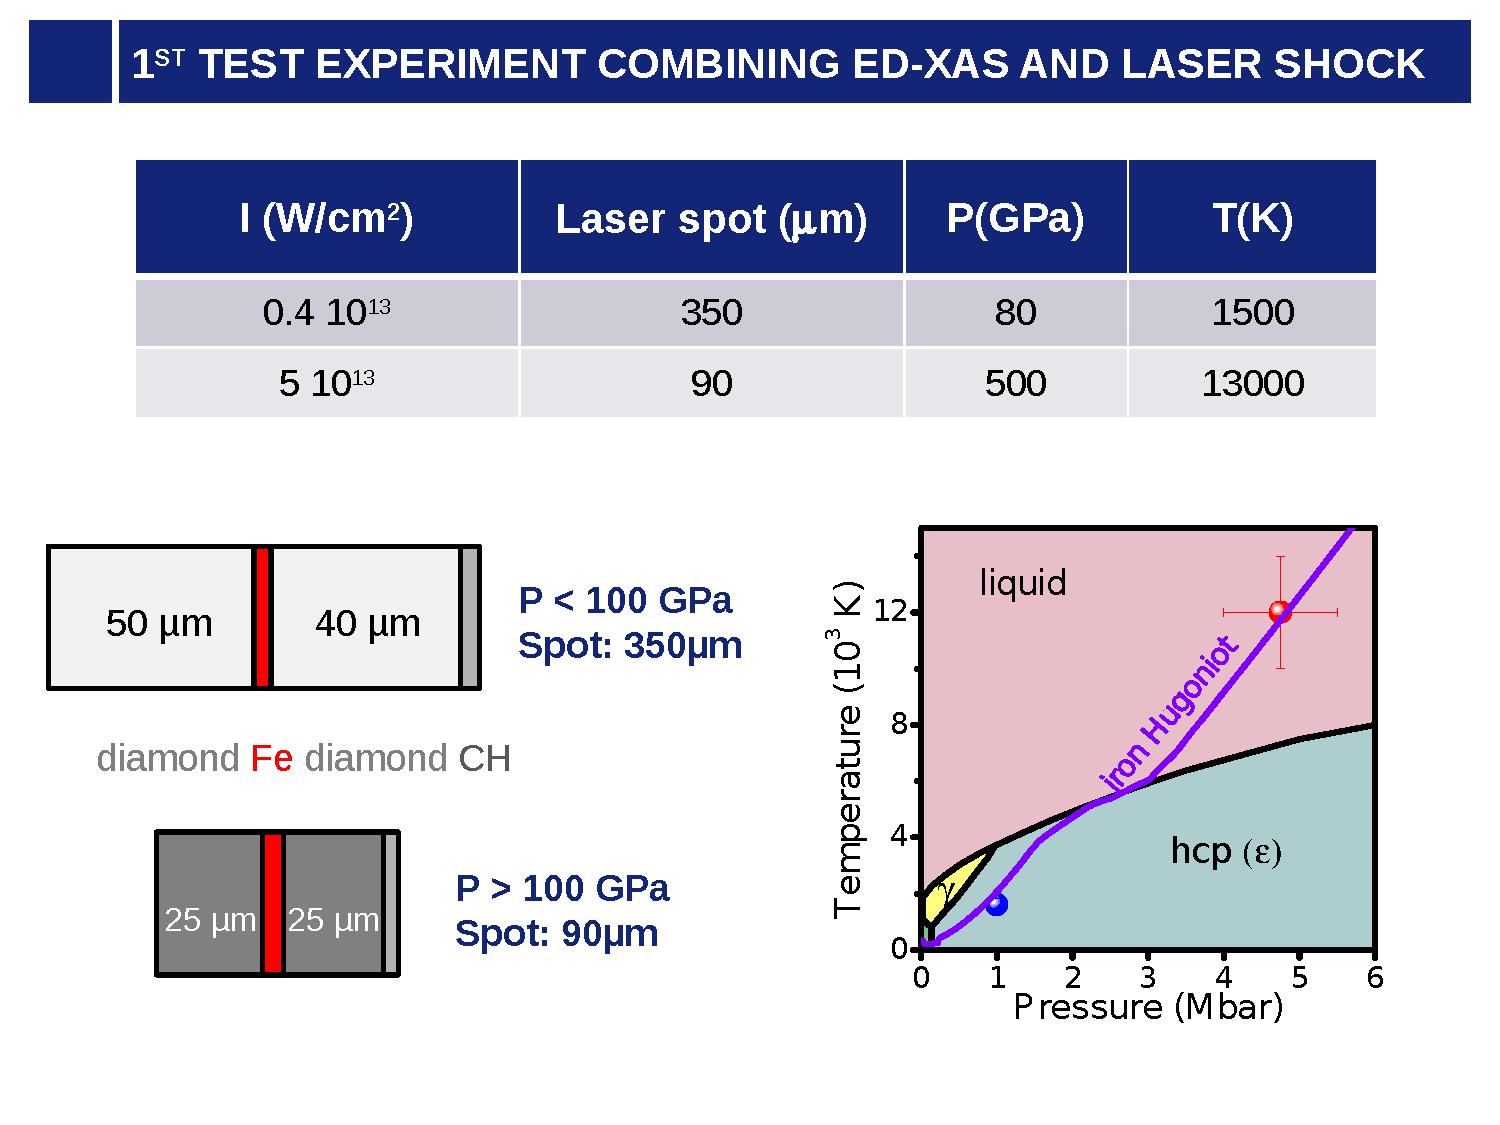
\includegraphics[width=0.45\colwidth,angle=0,clip, bb=0 0 700 470]{esrf_Fe_targets_eos}%
    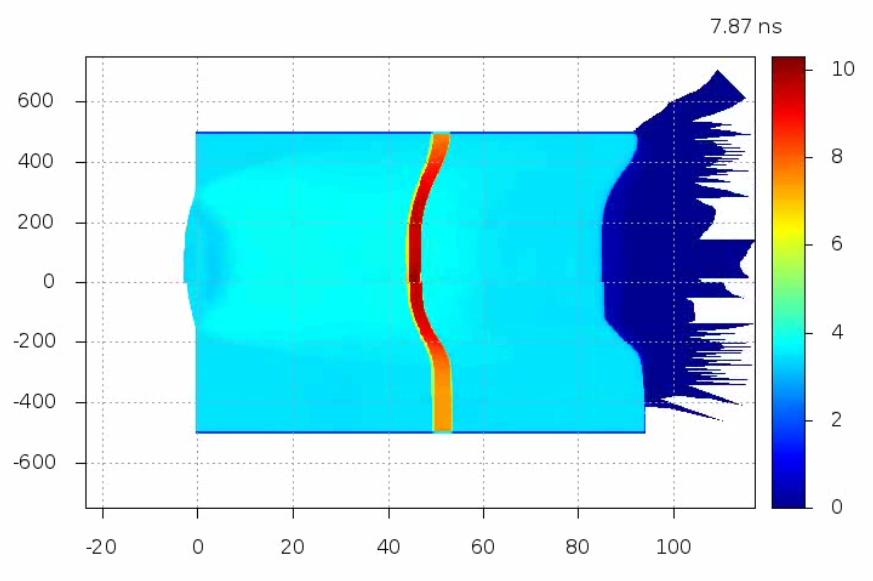
\includegraphics[width=0.45\colwidth,angle=0,clip]{esrf_Fe_sandwich_hydrosim}\\
    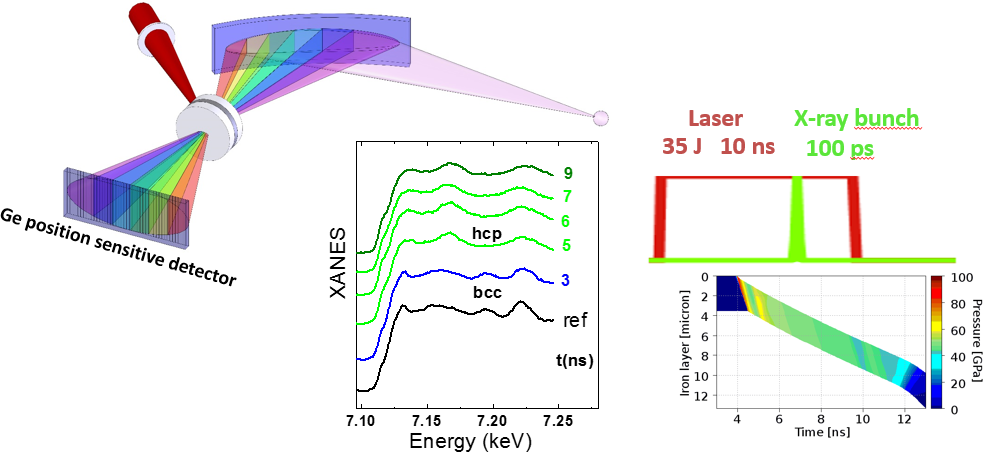
\includegraphics[width=0.8\colwidth,angle=0,clip]{esrf_Fe_xas_position}
  \end{center}
  }
}
\end{columns}
\begin{columns}
  \column{0.2}
  \useblockstyle{EucallLeft}
  % ESRF beam propagation
\block[bodyoffsetx=-15pt,titleoffsetx=-10pt]{Synchrotron simulations}{%
\begin{minipage}{.9\colwidth}%
  \mbox{}%
    \innerblock[titlewidth=\textwidth,bodywidth=\textwidth,titleleft, titleoffsetx=10pt,
    bodyoffsetx=10pt]
    {X-ray optics}
    {%
    \begin{center}
      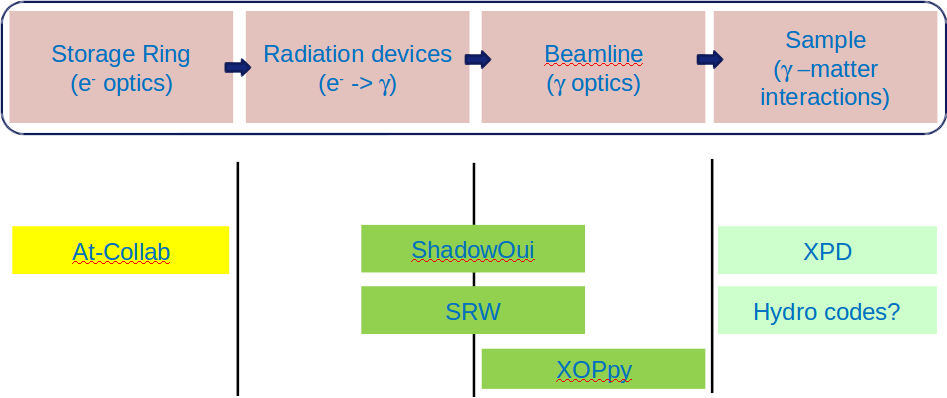
\includegraphics[width=.9\textwidth,angle=0,clip]{esrf_toolchain}
      \scriptsize\sf
      Propagation of synchrotron radiation and secondary particles to the sample interaction point.
    \end{center}
    }%
    \innerblock[titlewidth=\textwidth,bodywidth=\textwidth,titleleft, titleoffsetx=10pt,
    bodyoffsetx=10pt]
    {XPD shadowgraphy}{%
    \begin{center}
      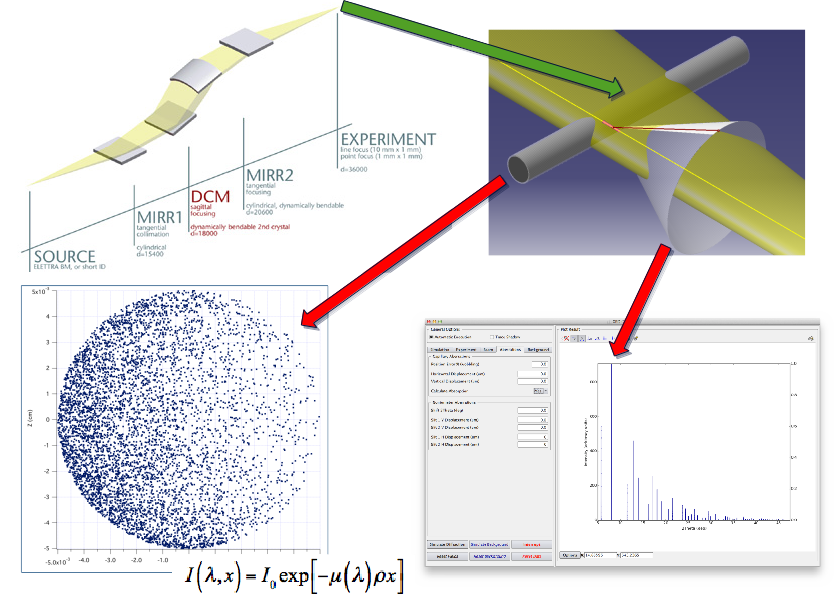
\includegraphics[width=.9\textwidth,angle=0,clip]{esrf_xpd_shadowgraphy}
    \end{center}
    }%
\end{minipage}
}
\column{0.6}
\useblockstyle{EucallCenter}
\block[bodyoffsetx=0pt]{Building a photon science simulation platform [4]}{%
\begin{center}
  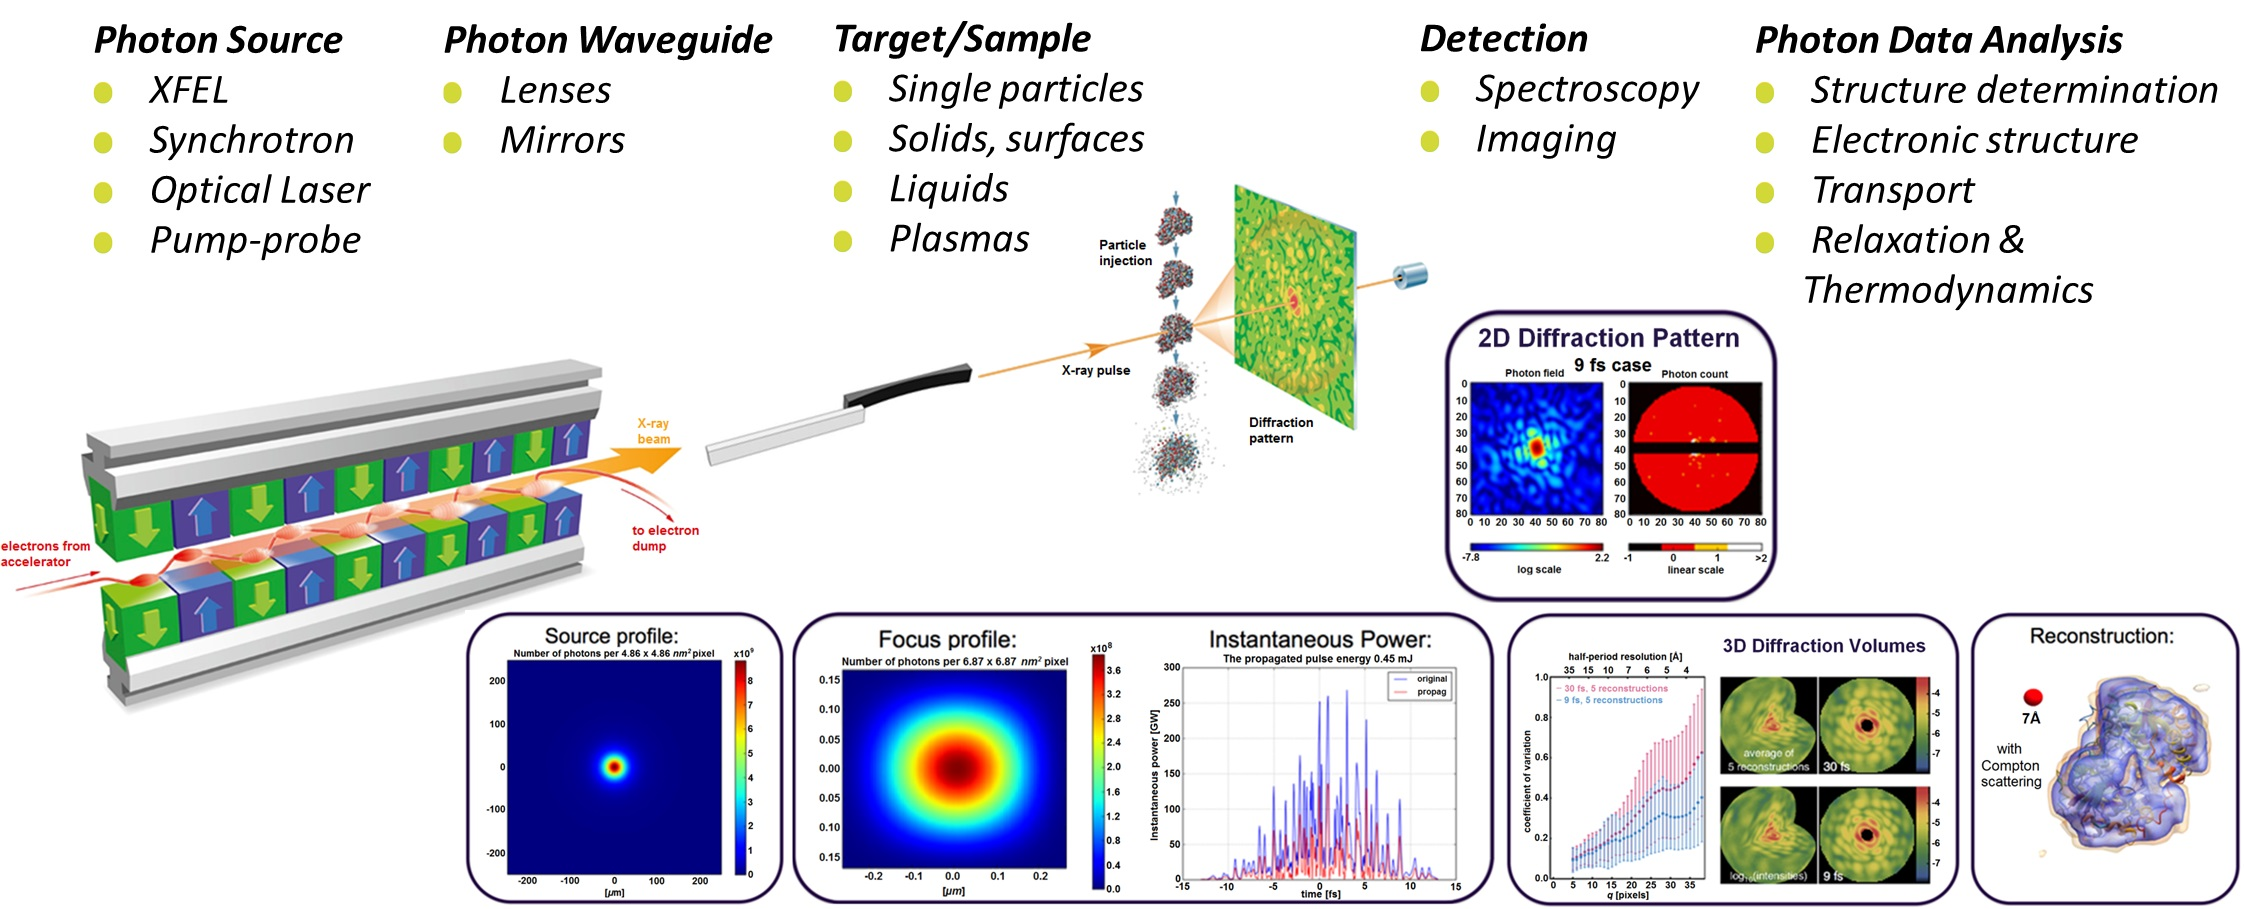
\includegraphics[height=0.19\textheight, width=0.95\colwidth,angle=0,clip]{simS2E_workflow}
\end{center}
}

\column{0.2}
  \useblockstyle{EucallRight}
% DESY HPC
\block[bodyoffsetx=-5pt]{DESY HPC infrastructure}{%
\begin{minipage}{.9\colwidth}%
  \mbox{}%
    \innerblock[titlewidth=\textwidth,bodywidth=\textwidth,titleleft, titleoffsetx=10pt,
    bodyoffsetx=10pt]
    {Current infrastructure}
    {%
      \begin{center}
      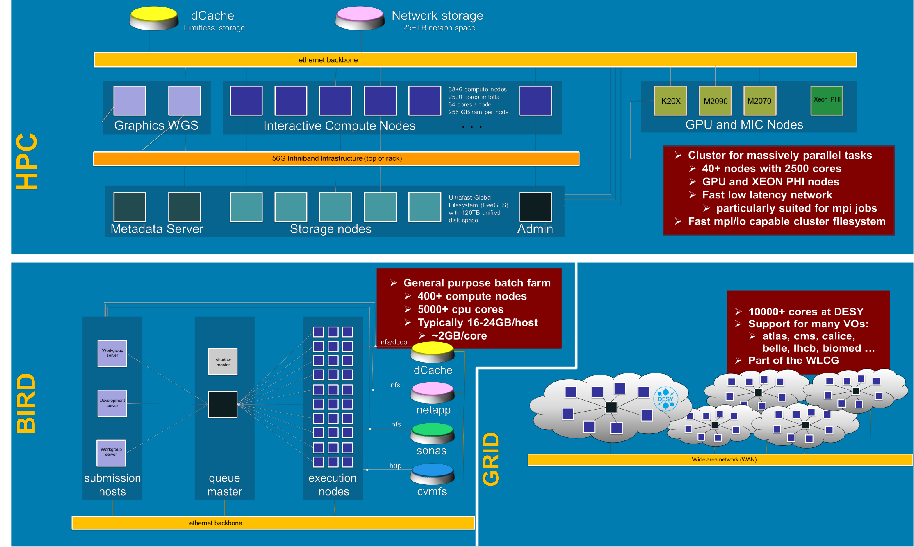
\includegraphics[width=.925\textwidth,angle=0,clip]{desy_hpc_status}%
      \end{center}
    }%
    \innerblock[titlewidth=\textwidth,bodywidth=\textwidth,titleleft, titleoffsetx=10pt,
    bodyoffsetx=10pt]
    {Future development} {%
    \begin{center}
      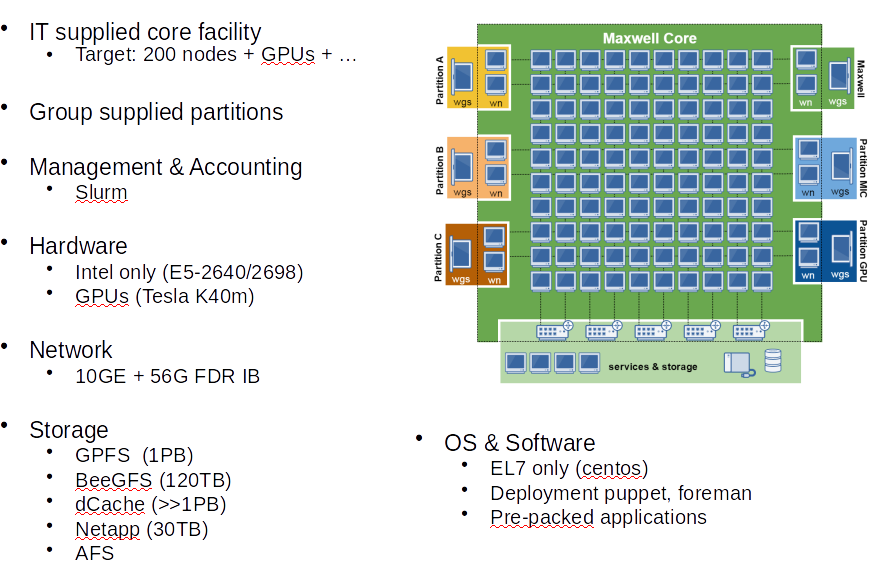
\includegraphics[width=.925\textwidth,angle=0,clip]{desy_hpc_future}%
    \end{center}
    }%
\end{minipage}
}
\end{columns}
\begin{columns}

%%%%%%%%%%%%%%% SECOND column
\column{0.5}
  \useblockstyle{EucallLeft}
% ELI-ALPS
\block{Radiation transport in complex targets [5,6]}{%
\begin{minipage}{.9\colwidth}%
  \mbox{}%
  \begin{minipage}[][.1\textheight][t]{.475\textwidth}%
    \innerblock[titlewidth=\textwidth,bodywidth=\textwidth,titleleft, titleoffsetx=10pt,
    bodyoffsetx=10pt]
    {Laser-plasma acceleration}
    {%
    \begin{center}
      \vspace*{1.45ex}
      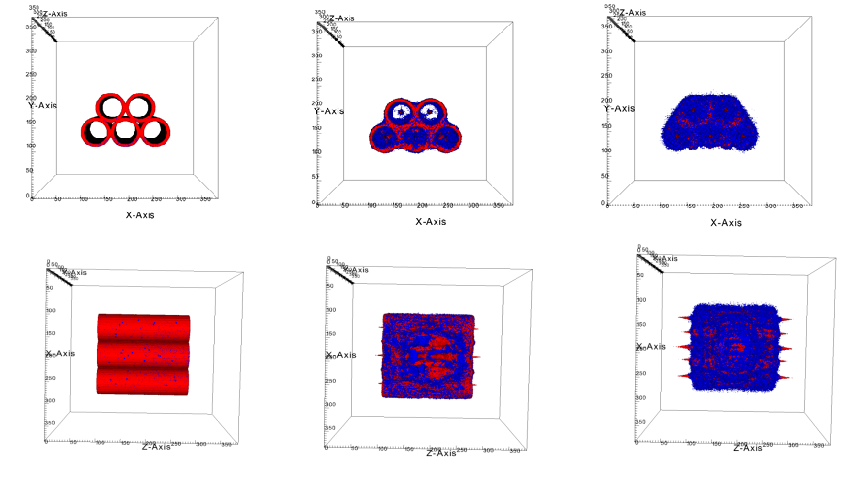
\includegraphics[width=0.95\textwidth,angle=0,clip]{eli-alps_e-ion_laser_acceleration.png}\\
      \scriptsize\sf
      Evolution of electron (blue) and ion (red)
      density distribution. Laser intensity $= 10^{20} W/cm^2$,  max. proton energy  = 40 MeV.\\
      \vspace*{1.45ex}
      {}
    \end{center}
    }%
  \end{minipage}
  \hfill%
  \begin{minipage}[][.1\textheight][t]{.475\textwidth}%
    \innerblock[titlewidth=\textwidth,bodywidth=\textwidth,titleleft, titleoffsetx=10pt,
    bodyoffsetx=10pt]
    {Electron transport in nanowires} {%
    \vspace*{1.55ex}
    \begin{center}
    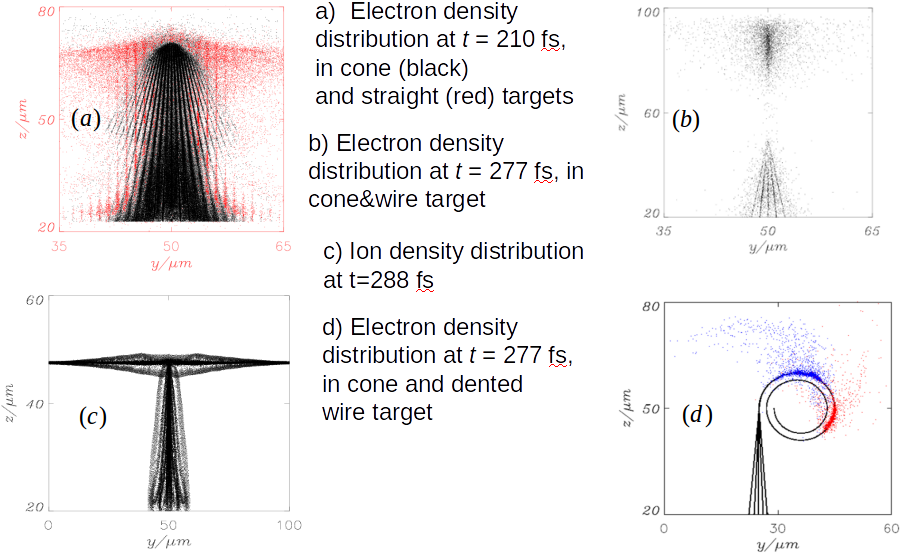
\includegraphics[width=0.95\textwidth,angle=0,clip]{eli-alps_wire_targets}
    \end{center}
    \vspace*{1.55ex}
    }%
  \end{minipage}
\end{minipage}
}
% ELI-NP
\column{0.5}
\useblockstyle{EucallRight}
\block{Secondary particle generation for nuclear physics [8]}{%
\begin{minipage}{.9\colwidth}%
  \mbox{}%
  \begin{minipage}[][.1\textheight][t]{.475\textwidth}%
    \innerblock[titlewidth=\textwidth,bodywidth=\textwidth,titleleft, titleoffsetx=10pt,
    bodyoffsetx=10pt]
    {ELI-NP facility and beamlines}
    {%
      \vspace*{1.65ex}
      \begin{center}
      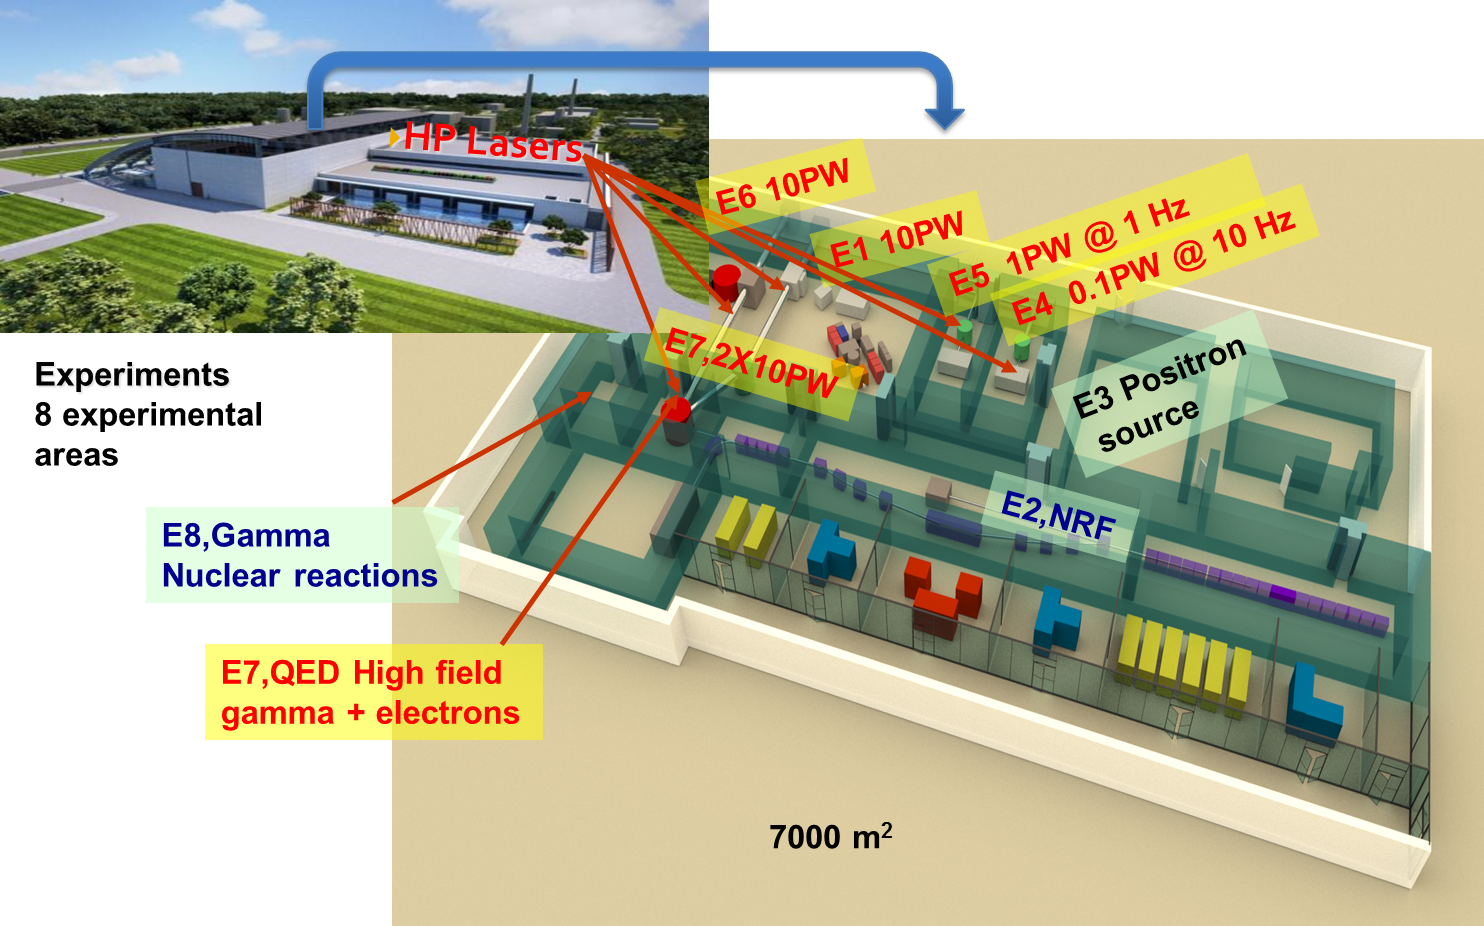
\includegraphics[width=.925\textwidth,angle=0,clip]{eli-np_model.png}%
      \end{center}
      \vspace*{1.65ex}
    }%
  \end{minipage}
  \hfill%
  \begin{minipage}[][.1\textheight][t]{.475\textwidth}%
    \innerblock[titlewidth=\textwidth,bodywidth=\textwidth,titleleft, titleoffsetx=10pt,
    bodyoffsetx=10pt]
    {Secondary particles tracking} {%
    \begin{center}
      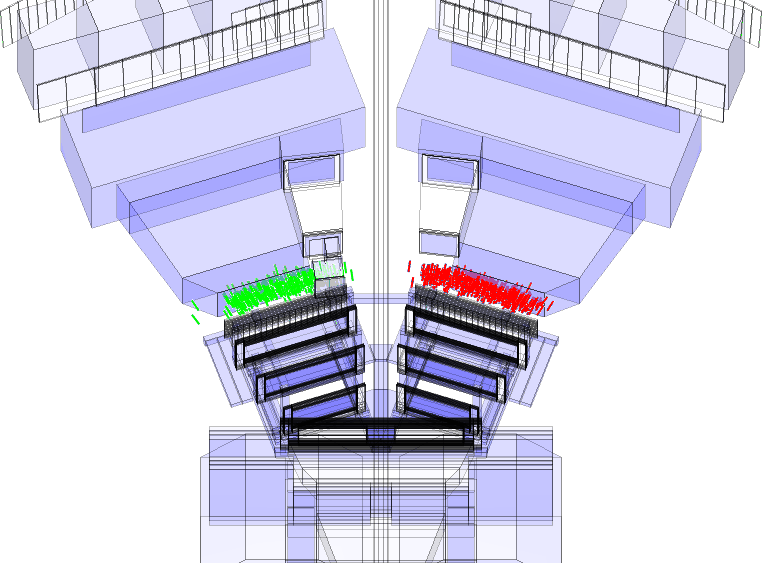
\includegraphics[width=.925\textwidth,angle=0,clip]{eli-np_sim_00080}
    \end{center}
    }%
  \end{minipage}
\end{minipage}
}
\end{columns}
\block{}{%
\begin{tikzpicture}%
  \draw (0,0) -- ( \textwidth - 4.5cm, 0);
\end{tikzpicture}\\[1ex]
\mbox{}
\begin{minipage}[][][t]{0.25\textwidth}%
  \noindent%
  {\sf%
  Contact: carsten.grote@xfel.eu\\%
  \noindent%
  Webpage: www.eucall.eu\\[2ex]
  }%
  \begin{minipage}{0.2\textwidth}%
    \includegraphics[width=1.0\textwidth]{eu_flag}%
  \end{minipage}%
  \hfill%
  \begin{minipage}{0.79\textwidth}%
    \small
  This project has received funding from the \textit{European Union's Horizon 2020 research and
  innovation programme} under grant agreement No 654220.\\
  \end{minipage}%
\end{minipage}%
%\hfill%
\begin{minipage}[][][t]{0.345\textwidth}%
  \includegraphics[width=\textwidth,angle=0,clip]{eucall_institutes}%
\end{minipage}%
\hfill%
\begin{minipage}[][][t]{0.345\textwidth}
  \small
  \underline{References}
  \begin{enumerate}
    \item Burau et al. IEEE Trans. Plasma Sc. \textbf{38} (2010).
    \item Chung et al, High Energy Dens. Phys. \textbf{1} (2005).
    \item
    \item Yoon et al. submitted.
    \item Lecz et al. Phys. Plasma \textbf{22} (2015)
    \item Lecz et al. submitted
    \item
  \end{enumerate}
\end{minipage}
}

\end{document}



